\chapter{Procesamiento de Texto }
\label{cap_txt}
\section{Introducción}

Los libros contenidos en la colección  de arte mexicano tienen mucho texto que puede ser utilizado para descubrir patrones de asociación entre ellos. Éste capítulo describe los dos algoritmos básicos utilizados para encontrar dicha estructura. El primero agrupa los libros por tópicos (términos) similares y el segundo encuentra grupos de libros similares. En concreto:

\begin{enumerate}
%\def\labelenumi{\arabic{enumi}.}
%\itemsep1pt\parskip0pt\parsep0pt
\item
  Se genera grupos por tópicos relevantes automáticamente usando el algoritmo
  \emph{LDA} (\emph{Latent Dirichlet Allocation}).
\item
  Se crea una medida de similitud entre documentos utilizando las técnicas \emph{TF-IDF} (\emph{Term Frequency - Inverse Document Frequency}) junto con \emph{LSI} (\emph{Latent Semantic Indexing}) para encontrar los más parecidos a cada libro.

\end{enumerate}

\begin{figure}[H]
\centering
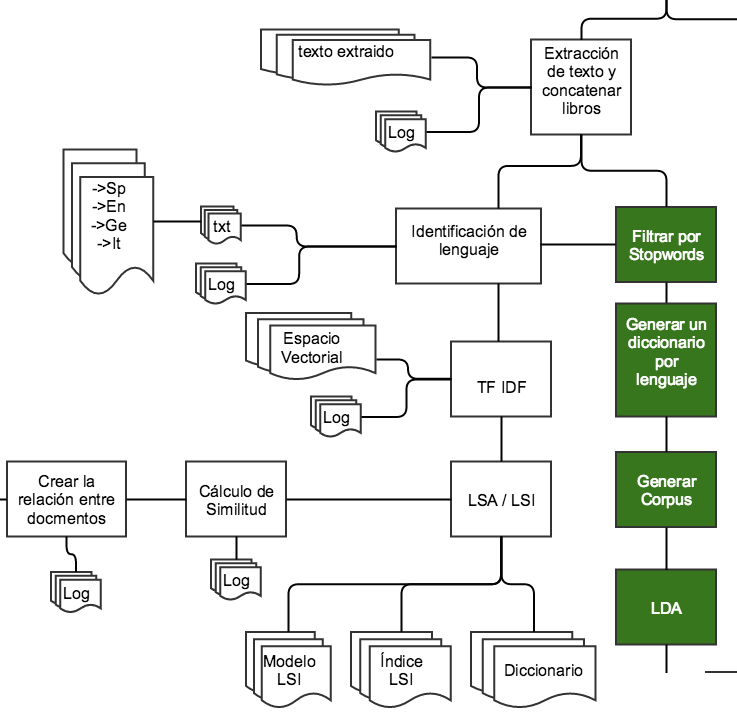
\includegraphics[width=0.6\textwidth]{Figures/pipeline_text.png}
\caption{Pipeline procesamiento de texto}
\end{figure}

La idea es que el usuario pueda explorar la colección de una manera más amigable que un simple listado de  libros. Los resultados del LDA permiten explorar grupos de libros similares a través  términos comunes entre ellos, mientras que el análisis de similitudes (TF-IDF) permite encontrar rápidamente los libros de la colección que sean parecidos al elegido inicialmente.

En principio, estos procesos serán completamente automáticos (salvo la elección de algunos parámetros descritos posteriormente) y le ahorrarán mucho tiempo a los expertos. En las siguientes secciones de este capítulo se describen a más detalle todos los componentes.\\

\textbf{Nota:} Tanto el equipo de la UNAM/ GIL como el equipo del ITAM usaron TF-IFD, dado que el equipo de la UNAM son los expertos en Lenguaje Natural se decidió utilizar el suyo en el flujo del proyecto.

\section{Vectorización de textos}

Antes de hacer los modelos es necesario convertir los datos no estructurados (es decir, los textos crudos de los libros) en datos estructurados. La técnica más común en minería de textos consiste en realizar conteos de palabras por documento y acomodarlos en una matriz. Conceptualmente, se construye la \emph{matriz términos-documentos} (TDM) $T$ como una matriz de entradas enteras de dimensión \emph{número de términos o palabras ($M$)} $\times$ \emph{número de documentos ($N$)}, con entradas:

$$
T_{w,d} = \text{número de veces que aparece el término } w \text{ en el documento (libro) } d
$$

Con la creación de la TDM se pierde el orden de las palabras en los libros, pero se mantiene la información estadística de las apariciones de las mismas. En principio, el número de términos debe coincidir con el número de palabras observadas en la colección, pero esto hace ruidosa la búsqueda ya que contabiliza todos los tiempos de los verbos. Por ejemplo, en este caso no se toma en cuenta que las palabras ``comer'', ``comen'' y ``comemos'' en realidad significan lo mismo y deberían tomarse en cuenta como una aparición del verbo ``comer''. Para tratar con este problema se hizo lo siguiente:

\begin{enumerate}
    \item Se separó la colección en varias subcolecciones, una por cada idioma disponible. Esto tiene sentido porqué cualquier asociación encontrada entre libros en diferentes idiomas puede ser considerada ruido y además puede hacer más lento el análisis. Todos los procesos subsecuentes se hicieron por separado en cada idioma.
    \item Se aplicó la técnica \emph{stemming} para disminuir el ruido de los términos, esta técnica consiste en utilizar la raíz de la palabra en lugar de la palabra misma, en el ejemplo de ``comer'', ``comen'' y ``comemos'' las contabiliza como la misma palabra (raíz ``come''). Hay varios algoritmos que hacen esto, pero dado el tamaño de la colección y por sugerencia del equipo de la UNAM, se hizo un \emph{stemming} simple truncando las palabras a una longitud máxima de 6 caracteres.
\end{enumerate}

De este modo, la TDM $T^{idioma_i}$ en realidad tiene un renglón por cada término de a lo más 6 letras encontrado en la colección en el $idioma_i$. 

\textbf{Nota:}En lo sucesivo se omitirá el idioma para facilitar la exposición, pero debe sobre entenderse que los análisis se hicieron por separado.

\section{Term Frequency – Inverse Document Frequency (TF-IDF) }

Para obtener una medida de similitud entre los documentos se aplicaron varias técnicas. En esta sección se explica la primera, que consiste en una transformación de la matriz $T$ para obtener similitudes. Para simplificar la notación, denotaremos por $T_d$ al vector de todas las frecuencias de los términos conocidos del documento $d$ y por $T_{w,d}$ las entradas de $T$ como están definidas en la sección anterior.

Supongamos que queremos comparar los documentos $q$ y $d$. Un primer enfoque que podríamos utilizar sería usar la similitud coseno, que toma en cuenta únicamente la frecuencia relativa de las palabras dentro de los documentos:

$$
sim(q,d) = \frac{T_q \cdot T_d}{\|T_q\| \|T_d\|}
$$

El problema con lo anterior es que las palabras comunes podrían tomar un papel fundamental y en nuestro caso compartir, por ejemplo, artículos o preposiciones no es muy interesante. Para mitigar esto se utilizó la frecuencia inversa en documentos $idf_w$, definida para una palabra $w$ como sigue: si $N$ es el número total de documentos en la colección y $df_w$ es el número de documentos de la colección que contienen a $w$, entonces definimos la frecuencia inversa de documentos como sigue:

$$
idf_w = log(\frac{N}{df_w}) 
$$

Entonces, en lugar de describir a $d$ por medio de $T_d$, lo describimos por medio de $c_d$, donde

$$
c_{d,w} = idf_w \times T_{d,w}
$$

Y así, calculamos la similitud entre dos documentos como el coseno entre sus vectores característicos:

\begin{align} \label{f:simcos}
sim(q,d) = \frac{c_q \cdot c_d}{\|c_q\| \|c_d\|}
\end{align}

La $idf_w$ es el logaritmo del inverso de la probabilidad de que el término $w$ aparezca en un documento elegido al azar. 
Las consecuencias de esto es que las palabras comunes casi no tendrán ningún efecto en la distancia, puesto que su probabilidad es cercana a 1 y por lo tanto su $idf$ es cercana a cero. 

Por el contrario, las palabras raras tendrán una probabilidad cercana a 0, por lo que su $idf$ será grande y contribuirán mucho. 
La idea detrás de este proceso es que se quiere que se utilice las palabras especiales o específicas a un contexto para discriminar, no las genéricas.
El esquema expuesto está escrito con mayor detalle en el libro \href{http://www.mmds.org}{Mining of Massive Datasets} ver \citep{leskovec2014mining},
con la pequeña diferencia de que nosotros no normalizamos $T_w$ por la máxima frecuencia obtenida por el término en la colección de documentos.


%%%% cambiar redacción 
Si bien se obtiene mucho mejores resultados utilizando la matriz $C = [c_1, \dots, c_N]$ es mucho más eficaz que si se utiliza la matriz $T$, aún hay ciertos elementos ruidosos que se puede mitigar. Para ello presentaremos la siguiente técnica.

\section{Latent Semantic Indexing (LSI)}

El Análisis de Semántica Latente (o LSI por sus siglas en inglés) es una técnica que se puede utilizar para refinar  más la similitud entre documentos calculada con TF-IDF.
Principalmente lo que hace es quitar el ruido de las palabras con muchos significados y de los términos con el mismo significado.
Para ello, encuentra los términos latentes u ocultos que conceptualmente tienen la mayor cantidad de información 
posible y los utiliza en lugar de las palabras normales.

Esta técnica fue propuesta por la UNAM y está explicada con mayor detalle en su documentación hermana, 
la idea general consiste en obtener la Descomposición en Valores Singulares (SVD) 
de la matriz TF-IDF y truncar los valores singulares pequeños,
dejando únicamente un número pequeño en comparación con el rango de la matriz (digamos, algún número entre 100 y 300).
Expresado matematicamente si la SVD de $C$ es 
$C = U \Sigma V^T$ \\

y $\Sigma_k = \Sigma$\\

una vez que se truncaron a cero todos sus valores singulares, a excepción de los $k$ más grandes, 
entonces se puede aproximar $C$ con $C_k = U \Sigma_k V^T$, donde
$C_k$ tiene rango $k \leq rango(C)$ y, por lo tanto, menos
efectos ruidosos que $C$. El LSI consiste en calcular las
similitudes como en la ecuación (\ref{f:simcos}), pero 
utilizando la matriz $C_k$ en lugar de $C$. En \citep{rosario2000} viene el proceso con más detalle.

Un factor importante para que funcione el LSI es el número de dimensiones latentes $k$ a utilizar. 
De preferencia debe ser elegido mediante validación por un
experto, que pueda evaluar los resultados obtenidos con diversos
valores de $k$ y elegir el que dé similitudes más coherentes. 
En la sección de resultados está explicado qué hace el programa para ayudar al experto a elegir $k$ de manera apropiada.


\section{Latent Dirichlet Allocation (LDA)}

A través de modelación de tópicos es posible analizar grandes cantidades
de datos sin categorizar cada uno por separado. Uno de los métodos más populares modelar tópicos es
LDA (Latent Dirichlet Allocation)  por sus cifras en inglés.
Es importante mencionar la propiedad de conjugación dadas las siguientes
distribuciones: Si tenemos:

\[ \phi \sim Dir(\alpha) \] \[ W \sim Mult(\phi) \] y
\[ n_k = |\{w_i:w_i = k \}| \] entonces
\[ P(\phi|\alpha, W) \propto P(W|\phi)P(\phi|\alpha) \]
\[ \propto \prod_k \phi^{n_k} \prod_k \phi^{\alpha_k-1} \]
\[ \propto \prod_k \phi^{\alpha_k+n_k-1} \]

Es decir son conjugadas, por lo que la distribución posterior tiene la
misma forma que la distribución a priori y en nuestro caso sólo estamos
agregando las observaciones. Ahora es más sencillo comprender la función
de LDA, el cual es un modelo generativo que asume:

\begin{enumerate}
  \item Cada tópico $k \epsilon \{1,...,K\}$ es una mezcla de palabras que tiene una distribución multinomial $\beta_k$ la cual proviene de una distribución de Dirichlet con parámetro $\lambda$. 
    \item Cada documento $d \epsilon \{1,...,M\} $ es una mezcla de tópicos con distribución multinomial $\sigma_d$ la cual proviene de una distribución de Dirichlet con parámetro $\alpha$.
    \item Para cada palabra $n \epsilon \{1,...,N\}$, se selecciona un tópico escondido (variable latente) $Z_n$, los cuales provienen de una distribución multinomial parametrizada por $\theta$.
\end{enumerate}

El modelo está representado por la figura \ref{lda}:

\begin{figure}[H]
\centering
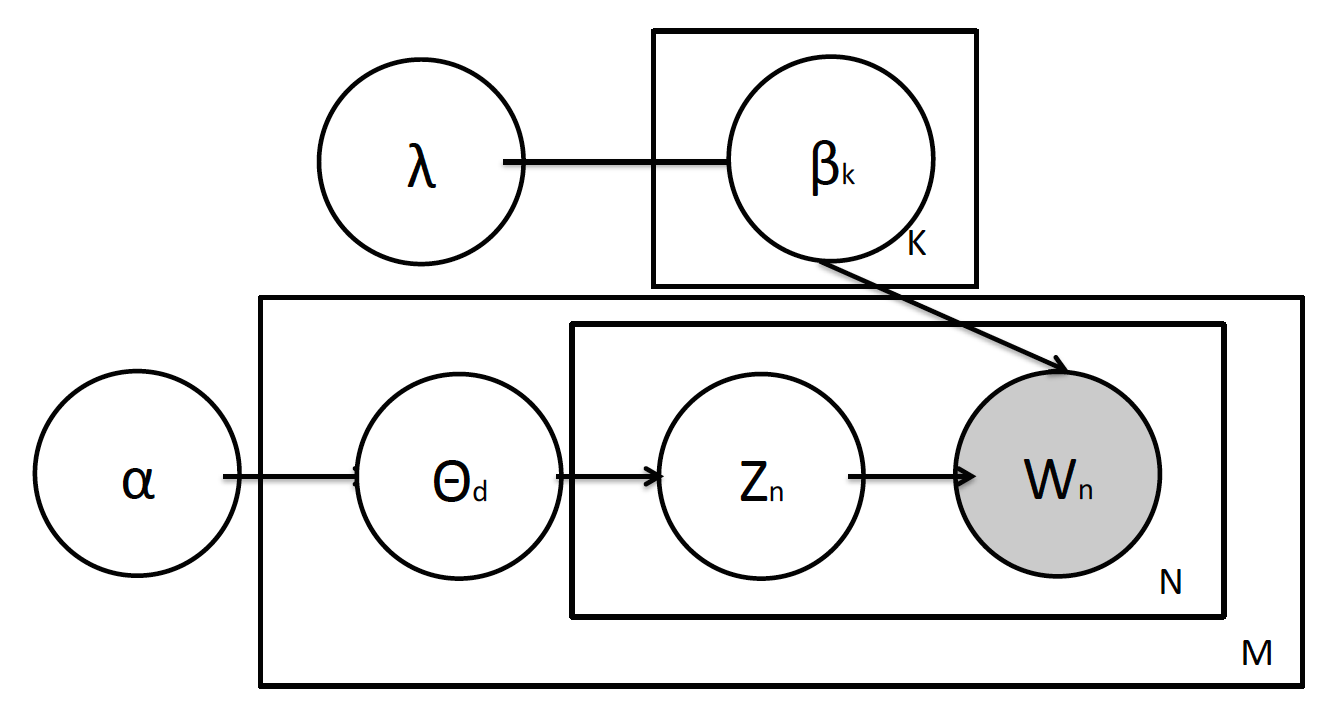
\includegraphics[width=.6\textwidth]{Figures/lda.png}
\caption{LDA}
\label{lda}
\end{figure}

Cada palabra observada está asociada con uno y sólo un tópico. Con base en esta idea y diagrama, es posible generar la palabra observada, es decir el tópico que le corresponde al documento.  A través de inferencia estadística descubriremos las variables latentes más probables, en nuestro diagrama las $Z_n$, las cuales explican de mejor manera nuestro conjunto de datos que nos va a decir cuáles son las $\beta_k$ y las $\theta_d$.
\vspace{0.5cm}

\noindent Para poder determinar los tópicos adecuados vamos a utilizar el muestreo de Gibbs (Gibbs sampling). Esto se logra a través de el cambio en la asignación de tópicos a cada una de las palabras $Z_{d,n}$ ya que comenzamos con asignaciones de tópicos de forma aleatoria y queremos ir mejorando estos tópicos de forma gradual hasta que tengan sentido. Es decir, dado un estado $\{Z_1, ..., Z_N\}$, tenemos que $Z_n \sim p(n_n|Z_1,...Z_{n-1}, Z_{n+1},..., Z_N, X,\Theta)$, y esto lo hacemos con repetición para todas las palabras en nuestros documentos.
\vspace{0.5cm}



\noindent Se inicia asignando tópicos a todas las palabras de todos los documentos y de forma sistemática se reasignan los tópicos a las palabras,  esto se hace de manera iterativa y cada vez se muestrea  la asignación de tópicos de una de las palabras basado en la asignación de las demás para todas las palabras, véase figura \ref{fig:Gibbs_sample}. Integrando al modelo las demás variables correspondientes a los parámetros $\alpha$ y $\lambda$ a través de Rao-Blackwellized \citep{Canini} ya que nos interesa:

\[ p(Z_{d,n}=k | Z_{-d,n}, w, \alpha, \lambda)= \frac{p(Z_{d,n}=k, Z_{-d,n}| w, \alpha, \lambda)}{p(Z_{d,n}| w, \alpha, \lambda)} \]


\vspace{0.5cm}

haciendo los  cálculos se tiene,

\[ p(Z_{d,n}=k | Z_{-d,n}, w, \alpha, \lambda)= \frac{n_{d,k}+\alpha_k}{\sum_{n=i}^{K}n_{d,i}+\alpha_i} \frac{v_{k,w_{d,n}}+\lambda_{w_{d,n}}}{\sum_i v_{k,i}+\lambda_i}\].



En dónde $n_{d,i}$ es el número de palabras que tienen el tópico $i$ en el documento $d$ y $v_{k,w}$ es el número de veces que la palabra $w$ se usa en el tópico $k$. Por lo que el proceso de remuestreo se puede dividir en dos partes y contar en dos partes:


\begin{figure}[h]\centering
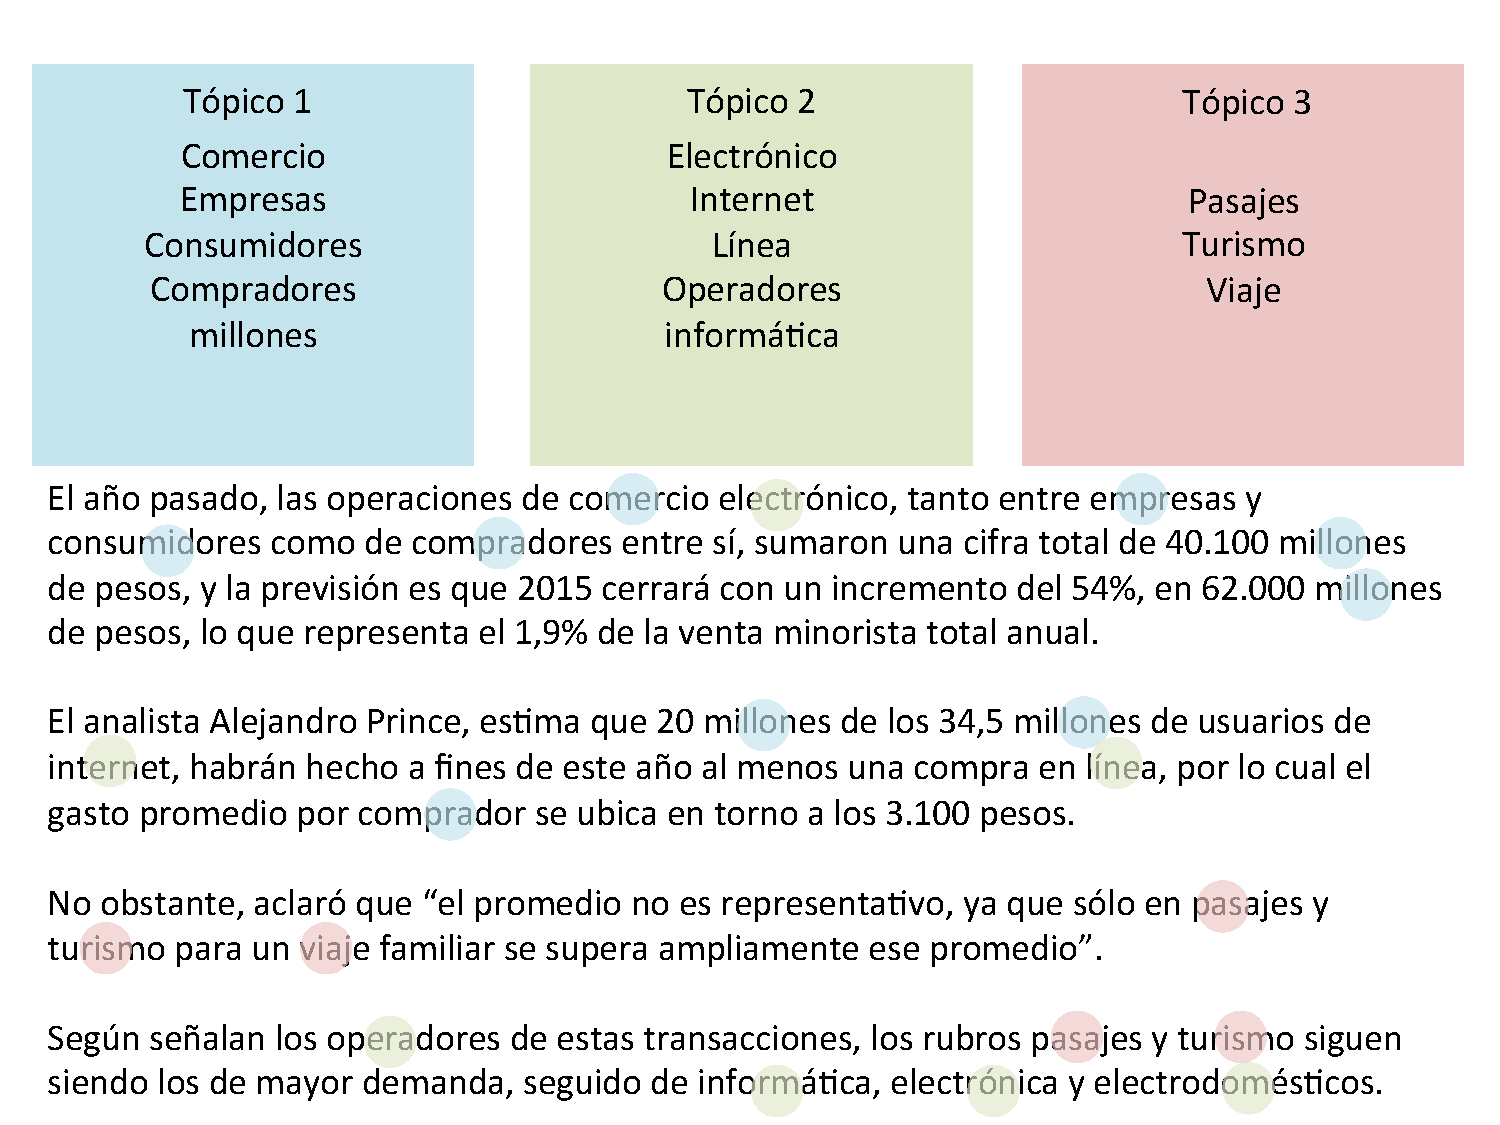
\includegraphics[width=12cm]{gibbs_sampling.pdf}
\caption{Muestreo de Gibbs}
\label{fig:Gibbs_sample}
\end{figure}

\newpage

\begin{enumerate}
  \item ¿Qué tantas veces aparece cada tópico en casa documento?
  \item ¿Qué tanto aparece cada palabra en cada tópico?
\end{enumerate}

Por lo que al multiplicar los valores obtenidos para cada una de las partes tenemos el valor proporcional de la probabilidad de asignación de los tópicos para la palabra que escogemos, y de esta manera vamos armando la mezcla de tópicos para cada documento, ver Figura \ref{fig:mezcla_topicos}


\begin{figure}[h]\centering
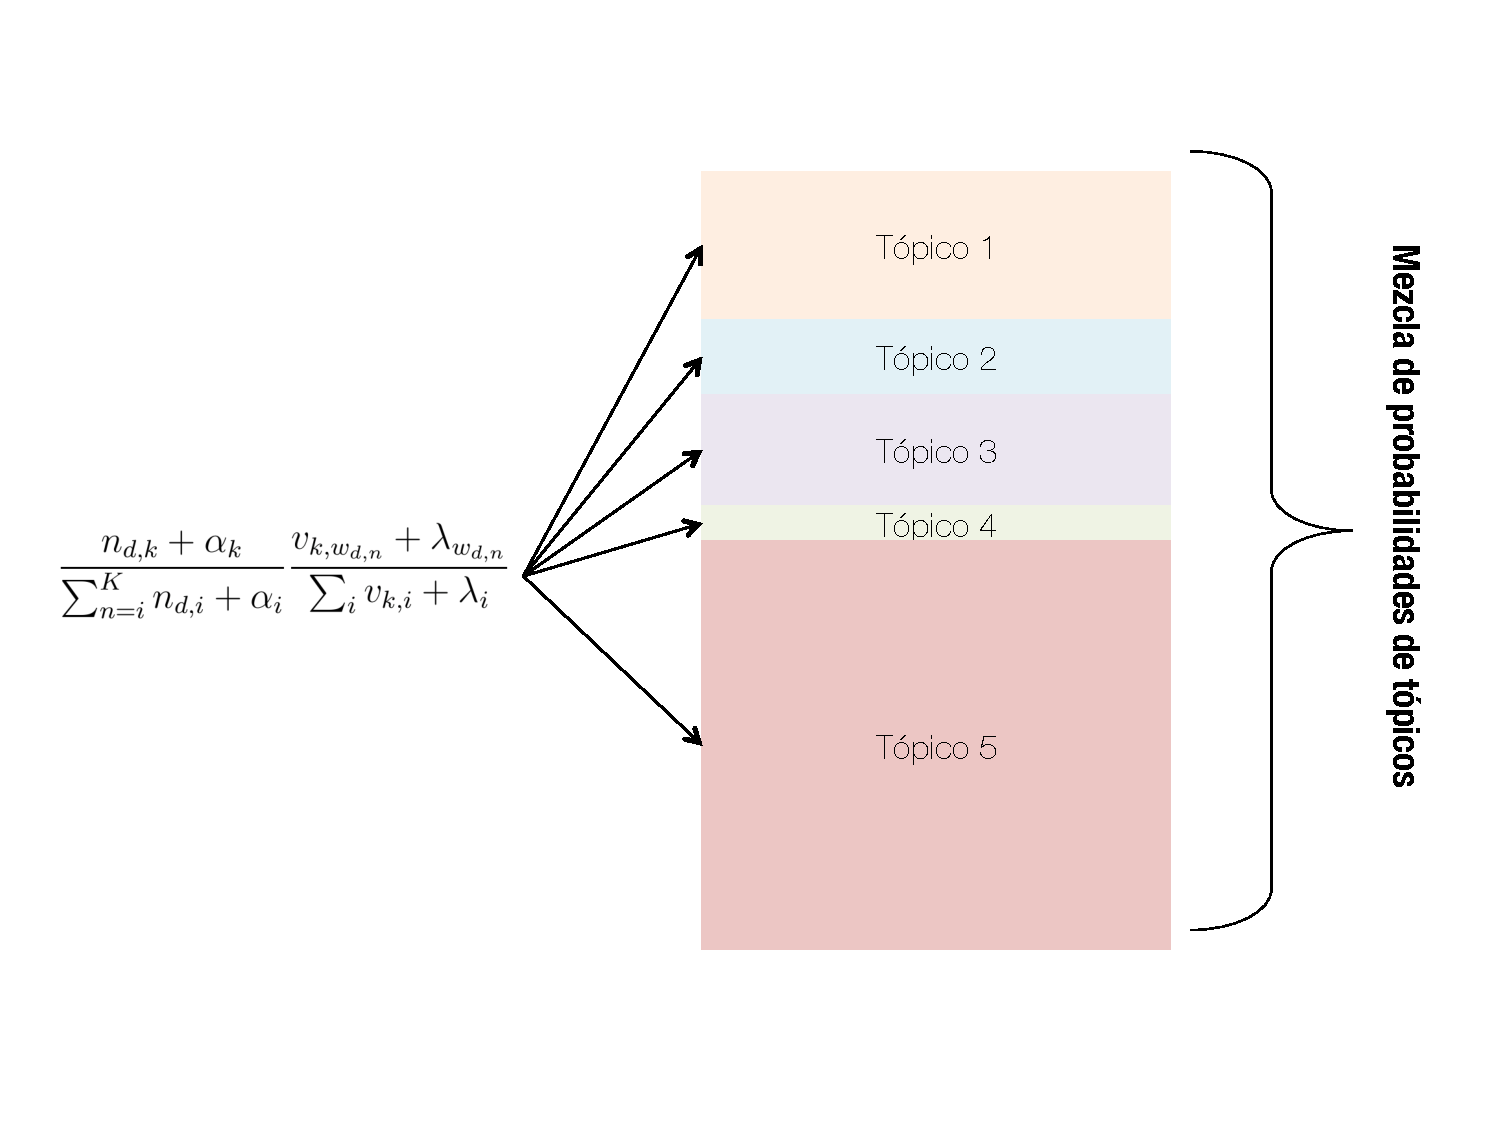
\includegraphics[width=12cm]{mezcla_topicos.pdf}
\caption{Mezcla de tópicos}
\label{fig:mezcla_topicos}
\end{figure}



\noindent El objetivo de encontrar los tópicos en la colección de texto es hacer una partición la cual nos permite identificar grandes bloques de temas. Esto se hace con el objetivo de poder buscar una colección o tema en particular dentro del catálogo. 



\section{Elección de parámetros} %No sabemos si es sección

En esta sección se explica el criterio para elegir los parámetros que permiten la implementación de distintos algoritmos los cuales son parte del pipeline. Existen parámetros que se deben elegir manualmente y se heredan a todos los procesos. 

\begin{itemize}
	\item Idiomas. 
	\item Nivel de limpieza.
\end{itemize} 

Es importante mencionar que se realiza la extracción y limpieza de todos los libros, y posteriormente sólo se realizan los modelos de los idiomas que se escogen.
\vspace{0.2cm}

\noindent Los parámetros a escoger que corresponden a LDA (modelación de tópicos automática) son:

\begin{itemize}
	\item Número de tópicos: Este parámetro corresponde a la cantidad de \textit{clusters} o nivel de partición del conjunto de libros. A mayor número de tópicos, mayor especificidad en  la asignación.
	\item El número de pasadas al texto: Este parámetro está implementado en el código, 
	sin embrago este es fijo a 10 ya que valores más altos implican un costo computacional más alto.
	Este parámetro puede ser explorado en un futuro para medir la ganancia en la especificidad de los tópicos.
\end{itemize}


Como se mencionó anteriormente un experto debe elegir los valores a utilizar. Para ayudarle a tomar la decisión, se generó un archivo en HTML que presenta los resultados como se muestra en la siguiente figura \ref{fig:outputLDA} :
\vspace{0.2cm}


\begin{figure}[h]\centering
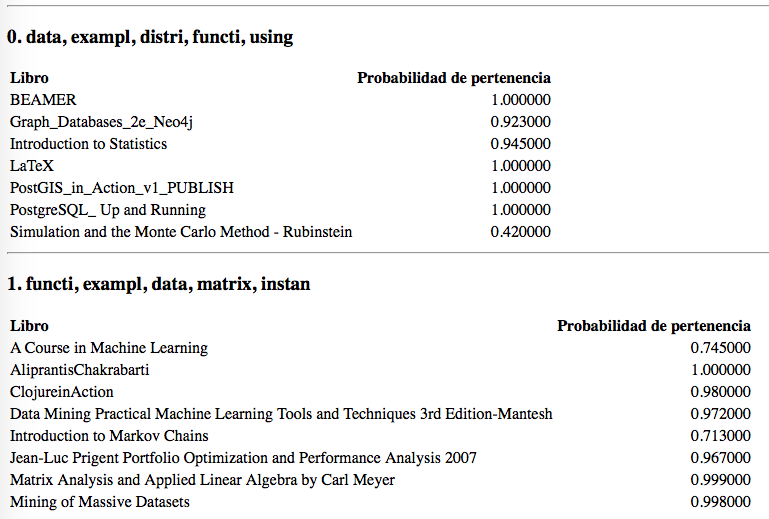
\includegraphics[width=5cm]{htmlLDA.png}
\caption{Salida en HTML de LDA}
\label{fig:outputLDA}
\end{figure}


\vspace{0.2cm}
El parámetro a escoger que corresponde a LSI (similitud entre libros) es:

\begin{itemize}
	\item Número de dimensiones latentes: Mientras más grande es este parámetro el criterio es más preciso, pero más ruidoso. Hay que probar varios valores para encontrar el nivel de especificidad óptimo. 
\end{itemize}


De manera similar presentamos los resultados en un archivo HTML el cual facilita la toma de decisión respecto al valor del parámetro mencionado anteriormente como se muestra en la siguiente figura \ref{fig:outputLSI}
\vspace{0.2cm}

\begin{figure}[h]\centering
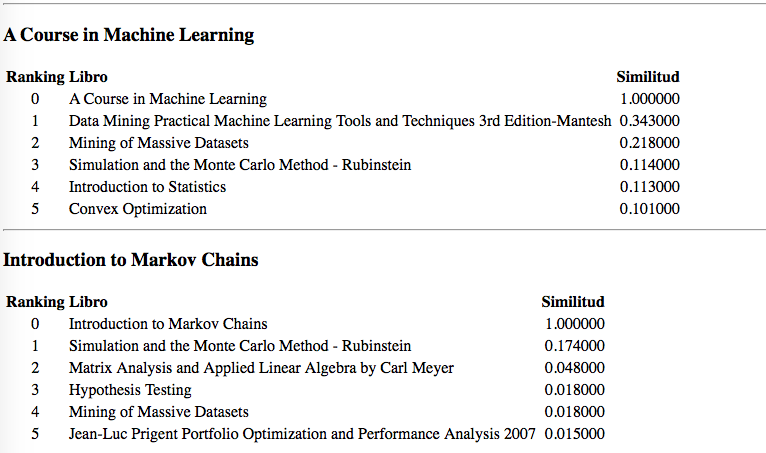
\includegraphics[width=5cm]{htmlLSI.png}
\caption{Salida en HTML de LSI}
\label{fig:outputLSI}
\end{figure}




\section{Conclusión}
El procesamiento de texto es sin duda, un análisis fundamental para encontrar patrones de asociación dentro de la colección de textos disponible y textos por agregar. Como se mencionó anteriormente, este proceso permitirá que el usuario pueda realizar búsquedas bajo distintos criterios ya sea por similitud en cuanto al texto, como lo permite la búsqueda por LSI, o en cuanto a temas en particular como lo permite la búsqueda por LDA.

El desarrollo del procesamiento de texto mediante una gestión de pipelines a través de \texttt{luigi} impulsa un ecosistema de producción sano, ya que existen procesos que por naturaleza son computacionalmente costosos y por lo tanto tardados los cuales pueden ser paralelizados y gestionados si es que existen errores. 
En particular dentro del pipeline de procesamiento de texto,  la limpieza es un proceso tardado, 
sin embargo con \texttt{luigi} es posible realizar esta tarea en paralelo y si existe un error en algún momento, no es necesario volver a generar toda la información desde cero, s
i no que retomamos el proceso a partir de dónde se generó el error. Por otra parte se genera la información necesaria una sola vez, la cual sirve para generar los modelos de LSI y LDA.

\section{Problemas}

Algunos de los mayores problemas encontrados a lo largo del desarrollo consistieron en el manejo de los hiper-parámetros del modelo, uno de estos consiste en el número de pasadas al texto el cual en cierto rango mejora el modelo. Este hiper-parámetro influye directamente con el tiempo de procesamiento de los datos. También se deja al criterio del usuario la selección del número de tópicos ya que esto depende del nivel de partición de la colección que se desee. Entre más tópicos, más específico es el subconjunto de selección, por esto es importante que el experto especifique el nivel de partición. Los tópicos están determinados por una combinación lineal en la que los escalares son la probabilidad de pertenencia de cada tema ($0.83 México + 0.65 dibujo + 0.55 paisaje + 0.5 Velasco$) . Es por esto que es importante que el experto determine un único tópico para esta combinación.

En general, el reto consistió en la construcción de un pipeline óptimo para el procesamiento de texto. Dado que existen procesos que tienen dependencias compartidas, fue fundamental la implementación a través de un esquema de pipelines como lo permite  \texttt{luigi} ya que se paralelizó el trabajo en ciertos procesos como lo fue la limpieza de datos y por otra parte se generó la información una única vez como lo es para el corpus y el diccionario, ya que estos fueron utilizados tanto para el desarrollo y generación de similitudes a través de LSI y el modelado de tópicos a través de LDA.

La presentación de resultados para la toma de decisión de los parámetros fue analizada y evaluada para ser presentada de forma sencilla ya que para el procesamiento interno solamente era necesario guardar los datos en una etapa del proceso en un formato de Python llamado \textit{pickle} el cual nos permite guardar los datos en forma binaria. Sin embargo, para conseguir un producto final en el que un experto determine los metaparámetros de los algoritmos, fue necesario determinar el formato más amigable para presentar los resultados obtenidos. En la sección \textit{Elección de parámetros} se menciona de forma detallada su interpretación. 

\section{Trabajo futuro}

Una manera de ampliar los resultados anteriormente expuestos, consiste en los siguiente:

\begin{enumerate}

	\item Reentrenamiento con datos nuevos: Por el momento es posible asignar una mezcla de tópicos a los documentos nuevos basado en el modelo LDA base. Sin embargo dado que la colección de textos incrementará con el tiempo, es altamente recomendado reentrenar el modelo de LDA ya que este contará con más información y probablemente con más tópicos. 
	\item Procesamiento en paralelo: A medida de que la colección crezca, es posible generar un modelo de LDA a través del procesamiento paralelo, esto con la finalidad de disminuir el tiempo de entrenamiento del modelo.
	\item Nuevas características y algoritmos: Dentro del procesamiento de texto es posible encontrar entidades véase \footcite{https://en.wikipedia.org/wiki/Named-entity_recognition}, por lo que se contempla en un futuro poder emplear este tipo de técnicas para encontrar relaciones entre entidades. 
	
\end{enumerate}

